\documentclass[12pt,a4paper]{article}  % шаблон для статьи, шрифт 12 пт
\usepackage[utf8x]{inputenc}  % использование кодировки Юникод UTF-8
\usepackage[russian]{babel}  % пакет поддержки русского языка
\usepackage{lipsum}  % Рыба-текст q
\usepackage[compact]{titlesec}  % для titlespacing
\titlespacing*{\section}{0.75cm}{1em}{0.1em}  % отступ заголовка 
% \titlespacing{\заголовок}{слева}{перед}{после}[справа]
\titlespacing*{\subsection}{0.75cm}{1em}{0.1em}
\usepackage{indentfirst}  % отступ первого абзаца
\setlength{\parindent}{0.75cm}
\usepackage[labelsep=endash]{caption}  % тире вместо двоеточия в картинках
\usepackage[labelsep=endash]{caption}  % тире вместо двоеточия в названиях 
\usepackage{graphicx}  % кртинки
\usepackage{comment}  % комментарии
\usepackage{tabularx}  % таблицы
\usepackage{color}  % цветной код
\usepackage{listings}  % листинги кода из файлов
\usepackage{cite}  % ???
\lstset{ %
	language=C++,                   % выбор языка для подсветки (здесь это С++)
	basicstyle=\small,              % размер и начертание шрифта для подсветки кода
	numbers=left,                   % где поставить нумерацию строк (слева\справа)
	numberstyle=\tiny,              % размер шрифта для номеров строк
	stepnumber=1,                   % размер шага между двумя номерами строк
	numbersep=5pt,                  % как далеко отстоят номера строк от подсвечиваемого кода
	backgroundcolor=\color{white},  % цвет фона подсветки - используем \usepackage{color}
	showspaces=false,               % показывать или нет пробелы специальными отступами
	showstringspaces=false,         % показывать или нет пробелы в строках
	showtabs=false,                 % показывать или нет табуляцию в строках
	frame=false,                    % рисовать рамку вокруг кода
	tabsize=2,                      % размер табуляции по умолчанию равен 2 пробелам
	captionpos=t,                   % позиция заголовка вверху [t] или внизу [b] 
	breaklines=true,                % автоматически переносить строки (да\нет)
	breakatwhitespace=false,        % переносить строки только если есть пробел
	escapeinside={\%*}{*)}          % если нужно добавить комментарии в коде
}

%перенос строк внутри таблиц
\newcommand{\specialcell}[2][c]{%
	\begin{tabular}[#1]{@{}c@{}}#2\end{tabular}}

\renewcommand\thefigure{\arabic{section}.\arabic{figure}}
%\renewcommand{\labelenumii}{\arabic{enumi}.\arabic{enumii}.} % Сквозная нумерация

\begin{document}

\thispagestyle{empty}

\begin{center}
\Large{
	\textbf{МИНОБРНАУКИ РОССИИ}
	
	\textbf{Санкт-Петербургский государственный}
	
	\textbf{электротехнический университет «ЛЭТИ»}
	
	\textbf{им. В.И. Ульянова (Ленина)}
	
	\textbf{Кафедра САПР}
}
\end{center}

\topskip=0pt
\vspace*{\fill}
\begin{center}
\Large{
	\textbf{
		КУРСОВАЯ РАБОТА\\
		по дисциплине «Программированние»\\
		Тема: Обработка текстовой информации\\
	}
}
\end{center}
\vspace*{\fill}

\begin{tabular}{lcr}
Студенты гр. 9892 & \begin{tabular}{p{60mm}} \\ \hline \end{tabular} & Лескин К.А.  \\\\ 
	              & \begin{tabular}{p{60mm}} \\ \hline \end{tabular} & Миллер В.В.  \\\\ 
Преподаватель     & \begin{tabular}{p{60mm}} \\ \hline \end{tabular} & Кузьмин С.А. \\\\
\end{tabular} 

\begin{center}
Санкт-Петербург\\
2020
\end{center}
%////////////////////////////////////////////////////////////////////////////////////////////////
%////////////////////////////////////////////////////////////////////////////////////////////////
%////////////////////////////////////////////////////////////////////////////////////////////////
\newpage

\begin{center}
	\Large{
		\textbf{Задание\\ на курсовую работу}
	}
\end{center}

Студенты Лескин К.А., Миллер В.В.\\

Группа 9892\\

Тема работы: Обработка текстовой информации\\

Исходные данные:

Разработать программу, осуществляющую обработку текстовой информации, согласно своему варианту задания.

Задачи данной курсовой работы включают выполнение следующих
этапов:\\
1) ввод исходного текста, хранящегося в виде файла;\\
2) ввод исходных данных для обработки текста (например, подстрока для
определения заданного места обработки; подстрока, соответствующая
заданной обработке; требуемые символьные данные; и т.п.);\\
3) обработку
текста,
соответствующую
индивидуальному
заданию
(опираясь на технику указателей и стандартные подпрограммы обработки
ASCII строк);\\
4) сохранение файла, соответствующего обработанному тексту;\\
5) вывод обработанного текста на экран.\\

Индивидуальный вариант задания:\\
В тексте, разделенном на слова, подсчитать количество
гласных и согласных. Упорядочить слова по содержащимся в них гласным
и/или согласным, а также по их относительному соотношению. Для слов
указать количество вхождений в текст.

%////////////////////////////////////////////////////////////////////////////////////////////////
%////////////////////////////////////////////////////////////////////////////////////////////////
%////////////////////////////////////////////////////////////////////////////////////////////////
\newpage

Содержание пояснительной записки:\\
Требуемые разделы пояснительной записки: «Содержание», «Введение», Основные главы,
«Заключение», «Список использованных источников».\\

Предполагаемый объем пояснительной записки:\\
Не менее 30 страниц.\\

Дата выдачи задания: %10.09.2019
\\

Дата сдачи реферата: %17.12.2019
\\

Дата защиты реферата: %24.12.2019
\\

\begin{tabular}{lcr}
	Студенты гр. 9892 & \begin{tabular}{p{60mm}} \\ \hline \end{tabular} & Лескин К.А.  \\\\ 
	                  & \begin{tabular}{p{60mm}} \\ \hline \end{tabular} & Миллер В.В.  \\\\ 
	Преподаватель     & \begin{tabular}{p{60mm}} \\ \hline \end{tabular} & Кузьмин С.А. \\\\
\end{tabular}

%////////////////////////////////////////////////////////////////////////////////////////////////
%////////////////////////////////////////////////////////////////////////////////////////////////
%////////////////////////////////////////////////////////////////////////////////////////////////

\newpage

\begin{center}
	\Large{
		\textbf{Аннотация}
	}
\end{center}

%Здесь своими словами нужно кратко описать выполняемую работу на
%русском и английском языках.

В данной курсовой работе необходимо реализовать программу, обрабатывающую текстовые данные, хранящиеся в виде файла, в соответствии с опцией, которую выбирает пользователь. Пользовательский интерфейс включает в себя меню, которое позволяет производить все необходимые манипуляции с исходными данными. Для выполнения данной курсовой работы будут использованы знания, полученные при выполнении лабораторных работ. В результате будет получена программа полностью соответствующая требованиям к индивидуальному заданию.
\\
\\
\\
\\
\\
\\
\\
\\
\\
\begin{center}
	\Large{
		\textbf{Summary}
	}
\end{center}

In this coursework, we need to implement a program that processes text data stored as a file, in accordance with the option that the user chooses. The user interface includes a menu that allows you to make all the necessary manipulations with the original data. In this coursework we will use the knowledge gained during laboratory work. As a result, the program will be fully compliant with the requirements for the individual task.

%////////////////////////////////////////////////////////////////////////////////////////////////
%////////////////////////////////////////////////////////////////////////////////////////////////
%////////////////////////////////////////////////////////////////////////////////////////////////
\newpage

\tableofcontents

%////////////////////////////////////////////////////////////////////////////////////////////////
%////////////////////////////////////////////////////////////////////////////////////////////////
%////////////////////////////////////////////////////////////////////////////////////////////////
\newpage

\section*{Введение}
\addcontentsline{toc}{section}{Введение}

Целью данной курсовой работы является углубление знаний в технологии программирования типовых задач
обработки текстовых данных.

В ходе выполнения работы мы воспользуемся всеми знаниями, полученными при выполнении лабораторных работ.
Содержание пояснительной записки к курсовой работе соответствует стандартным требованиям к пояснительным документам для программного продукта.

В данной курсовой работе предполагается использование функций для
работы со строками библиотеки <string> [1] и функции работы с файлами библиотеки <fstream> [2],
изученных в ходе выполнения
предыдущих лабораторных работ.
Ввод исходной строки осуществляется через внешний файл. 

Вывод полученной новой строки осуществляется в новый файл. 

Ввод других необходимых данных для выполнения программы (например, слов или же
отдельных символов) может осуществляться как через отдельный файл, так и
напрямую с консоли. При этом, необходимо вывести на консоль весь ход
выполнения программы (комментарии по действиям программы, копии
вводимых и выводимых данных).

При разработке программы необходимо учитывать и корректно
обрабатывать исключительные ситуации, которые могут возникнуть при
открытии для чтения или записи несуществующего файла.
Строки и слова в программе должны быть представлены с помощью
специального типа данных "string".

\begin{comment}
В этот раздел можно поместить копию цели и задания на курсовую
работу, а также указаний по её выполнению.
\end{comment}

%////////////////////////////////////////////////////////////////////////////////////////////////
%////////////////////////////////////////////////////////////////////////////////////////////////
%////////////////////////////////////////////////////////////////////////////////////////////////
\newpage

\section{Внешние форматы хранения данных}
\setcounter{figure}{0}
\begin{comment}
В этом разделе пояснительной записки нужно будет описать содержание
входных и выходных файлов, используемых в программе. При описании
нужно будет указать, из каких частей (компонент) состоит каждый файл и
где в нём будут располагаться требуемые данные.
\end{comment}
Входной файл может иметь любой формат, программа в любом случае его считает. Для примера и тестирования был создан файл bigfile без формата, содержащий текст на английском языке и включающий в себя занки препинания и пунктуации. 

Содержимое входного файла bigfile представленно на рисунке \ref{in_file}.


\begin{figure}[h!]
		\centering
		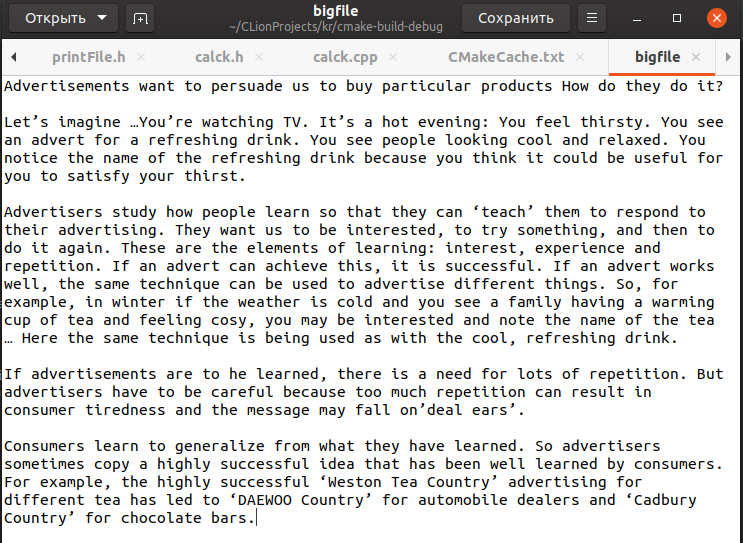
\includegraphics[width=0.9\linewidth]{photo/in_file}
		\caption{Входной файл bigfile}
		\label{in_file}
\end{figure}
%////////////////////////////////////////////////////////////////////////////////////////////////
%////////////////////////////////////////////////////////////////////////////////////////////////
%////////////////////////////////////////////////////////////////////////////////////////////////
\newpage
\section{Внутренние форматы хранения данных}
\setcounter{figure}{0}
\begin{comment}
В
этом
разделе
пояснительной
записки
нужно
будет
привести
графические рисунки, описывающие используемые структуры данных для
всех значимых переменных программы.
\end{comment}
Для хранения содержимого файла используется динамический массив, состоящий из слов типа std::string. Указатель на этот массив хранится в main и инициализируется при открытии файла. Каждая ячейка массива является объектом std::string и в свою очередь хранит своё слово в отдельности.

Схема хранения данных представленна на рисунке \ref{data_scheme}, где n --- количество слов в исходном файле.
\begin{figure}[h!]
	\centering
	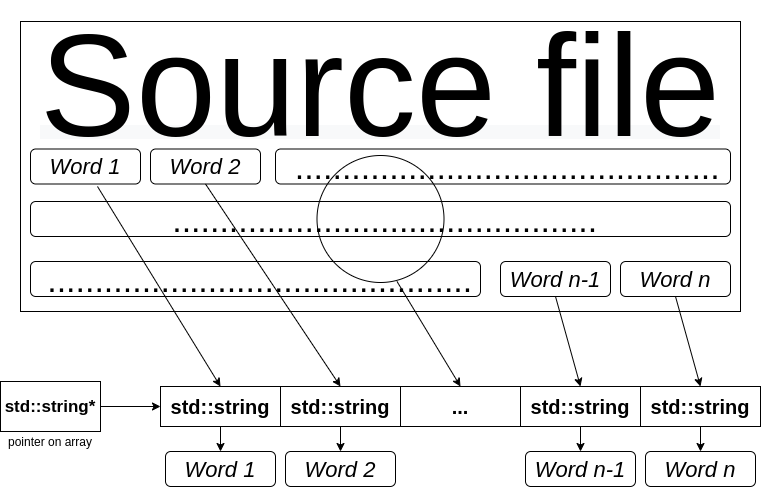
\includegraphics[width=0.9\linewidth]{photo/Scheme_of_data}
	\caption{Формат хранения данных, полученных из файла}
	\label{data_scheme}
	
\end{figure}

В данном контексте словом считается любая последовательность символов (от одного и больше), разделённая с двух сторон пробелами, либо символами табуляции (символ табуляции, символ переноса строки и пр.).
%////////////////////////////////////////////////////////////////////////////////////////////////
%////////////////////////////////////////////////////////////////////////////////////////////////
%////////////////////////////////////////////////////////////////////////////////////////////////
\newpage
\section{Описание пользовательских функций и модулей программы}
\setcounter{figure}{0}
\begin{comment}
В этом разделе отчёта нужно будет привести краткое описание
разработанных модулей программы, а также пользовательских функций и
методов в следующем формате (табл. 1):
Табл. 2 Описание модулей, структур/классов, функций/методов программы
Имя
Имя
Назначение
Параметры
Возвращаемое
модуля структуры/класса
для функции
функцией
или функции
значение
\end{comment}

Все функции и модули, реализованные в ходе выполнения данной курсовой работы, представленны в таблице \ref{funcsnmodules}.

\begin{table}[h!]
	\caption{Описание пользовательских функций и модулей программы}
	\label{funcsnmodules}
\begin{tabularx}{300pt}{|m{2,3 cm}|m{1,95 cm}|m{3 cm}|m{3 cm}|m {2,3 cm}|}
	\cline{1-5}
	Имя модуля & Имя функции & Назначение & Параметры функции & Возращаемое значение функции \\

	\cline{1-5} 
	openFile.h & openfile    & Открытие файла & int \&wordsSize, std::string \&name & std::string* \\ 
	
	\cline{1-5} 
	countVC.h & countVC & Подсчёт количества гласных и согласных в тексте & const std::string *words, int wordsSize, int \&V, int \&C, int \&N & void \\ 

	\cline{1-5} 
	writeFile.h & writeFile & Запись изменённого текста в файл & std::string *words, unsigned int wordsSize, char opt = '6' & void \\ 

	\cline{1-5} 
	countWords.h & countWords & Подсчёт количества слов в файле (без учёта повторений)& int wordsSize, std::string nameOfFile & bool \\ 
	
	\cline{1-5} 
	sortVC.h & sortVC & Сортировка слов в файле по заданным параметрам & std::string *words, const int \&wordsSize, char \&opt & void \\ 
	
	\cline{1-5} 
	printFile.h & printFile & Вывод содержимого файла на экран & const std::string *words, const int \&wordsSize & void \\ 
	
	\cline{1-5} 
	calck.h & calck & Подсчёт коэффициента слова по его гласным и согласным & const double \&v, const double \&c, const char \&opt & double \\ 
	\cline{1-5} 
\end{tabularx} 
%void writeFile(std::string *words, unsigned int wordsSize, char opt)
\end{table}
%////////////////////////////////////////////////////////////////////////////////////////////////
%////////////////////////////////////////////////////////////////////////////////////////////////
%////////////////////////////////////////////////////////////////////////////////////////////////
\newpage
\section{Описание интерфейса пользователя}
\setcounter{figure}{0}
\begin{comment}
	Здесь нужно привести фразы, которые выводятся на экране программы:
	какие данные программа просит пользователя ввести и в каком порядке, что
	происходит, если пользователь выберет тот или иной пункт меню и т.п.
\end{comment}
При запуске программы пользователю пердоставляется меню из девяти пунктов (рисунок \ref{main_menu}). 

\begin{figure}[h!]
	\centering
	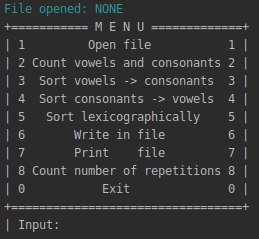
\includegraphics[width=0.7\linewidth]{photo/main_menu}
	\caption{Главное меню}
	\label{main_menu}
\end{figure}

Вверху меню отображается имя текущего файла. По умолчанию при окрытии файл не открыт, и показывается NONE.

При выборе пункта меню Open file на экран выводятся файлы текущей директории. Если введено ошибочное имя файла выводится сообщение об ошибке, в противном случае над меню вместо NONE отображается имя открытого файла.

Если никакой файл не открыт, выборы путктов 2-8 влекут за собой вывод сообщения о том, что файл не открыт.

При выборе 2 пункта Count vowels and consonants на экран выводится количество гласных и согласных букв в тексте файла, а так же количество символов, которые не являются буквами. Стоит отметить, что считаются только буквы латинского алфавита.

Выбор пунктов 3-5 приводит к выводу на экран сообщения, в какой файл были записаны изменения. При неудачной попытке будет выведено сообщение об ошибке.

Пункт 6 предлагает пользователю ввести имя файла, в который он хочет записать изменения. Если файл с таким именем существует, программа предупредит об этом и попросит пользователя подтвердить перезапись существующего файла.

Пункт 7 выводит содержимое файла на экран.

Пункт 8 выводит все уникальные (не повторяющиеся) слова в формате:\newline
[порядковый номер слова] [количесво повторов] [слово]\\
В конце списка выводится сообщение о количестве уникальных слов и самое часто встречающееся слово с количеством его повторений. Если все слова повторяются не более одного раза об этом будет выведено сообщение.

Выбор последнего пункта приводит к завершению программы с соответствующим сообщением.

Если пользовательский ввод содержит недопустимое значение, программа выведет сообщение о некоррктном вводе и вернёся в меню.
%////////////////////////////////////////////////////////////////////////////////////////////////
%////////////////////////////////////////////////////////////////////////////////////////////////
%////////////////////////////////////////////////////////////////////////////////////////////////
\newpage
\section{Описание алгоритма работы программы}
\setcounter{figure}{0}
\begin{comment}
	Здесь нужно на псевдокоде или же своими словами описать основные
	шаги и операции, что выполняет программа.
\end{comment}

\subsection*{Функция main}
\addcontentsline{toc}{subsection}{Функция main}

При запуске программы создаются переменные для хранения данных:
\begin{itemize}
	\item символ для хранения выбранного пункта меню;
	\item указатель на массив слов (в данном массиве хранятся слова из файла);
	\item имя текущего файла;
	\item количество слов в текущем файле;
	\item три ячейки для хранения количества гланых, согласных и не-букв в тексте файла;
\end{itemize}

Запускается цикл.

ПОКА выборанный пункт меню НЕ РАВНО '0'\\

Выводится имя открытого файла.

ЕСЛИ имя файла пустое ПЕЧАТЬ "NONE"

ИНАЧЕ ПЕЧАТЬ имя файла\\

Выводится текст меню.\\

ВВОД пункта меню\\

ЕСЛИ 1 
Удаляются все слова из массива. Счётчики букв устанавливаются в -1. Выводятся возможные файлы к открытию. Запускается функция openFile. Её возращаемое значение перезаётся указателю.

ЕСЛИ 2
Сначала проверяется, что в массиве есть слова. Для это смотрим на счётчик слов wordsSize. Потом проверяется, не посчитаны ли уже гласные и согласные. Для этого смотрим на счётчик гласных V. Если проверки прошли, запускается функция подсчёта countVC. В конце выводим сообщение с полученными данными.

ЕСЛИ 3
Сначала проверяется, что в массиве есть слова. Для это смотрим на счётчик слов wordsSize. Если слова есть, запускается функция sortVC.

ЕСЛИ 4
Сначала проверяется, что в массиве есть слова. Для это смотрим на счётчик слов wordsSize. Если слова есть, запускается функция sortVC.

ЕСЛИ 5
Сначала проверяется, что массив слов не пуст. Если слова есть, запускается функция std::sort из стандартной библиотеки STL, а изменения записываются в файл функцией writeFile. Инече выводится сообщение об ошибке.

ЕСЛИ 6
Сначала проверяется, что массив слов не пуст. Если слова есть, запускается функция writeFile. Инече выводится сообщение об ошибке.

ЕСЛИ 7
Запускается функция printFile.

ЕСЛИ 8
Запускается функция countWords.

ЕСЛИ 0
Программа завершается.

В остальных случаях выводится сообщение о неверном вводе.



\subsection*{Функция openFile}
\addcontentsline{toc}{subsection}{Функция openFile}

Проверяется входной параметр имени файла. Если он пустой, имя файла вводтся с клавиатуры. Иначе он сохраняется в локальную переменную. Открывается файл. В случае успеха выводится сообщение об успешном открытии и имя файла сохраняется в переменной, отвечающей за имя файла в функции main. Иначе выводится сообщение об ошибке и функция возвращает nullptr. Циклом проходимся по файлу и на каждое слово инкрементируем счётчик слов. Выделяем массив размером с количество слов в файле. Заново переоткрываем файл и считываем слова в массив. Закрываем файл и возвращаем указатель на созданный массив.

\subsection*{Функция countVC}
\addcontentsline{toc}{subsection}{Функция countVC}

\begin{itemize}
	\item Идём по всему массиву
	\subitem Идём по каждому символу в слове
	\subsubitem Если символ - гласная буква, увеличиваем счётчик гласных
	\subsubitem Если символ - буква, увеличиваем счётчик согласных
	\subsubitem Иначе увеличиваем счётчик не-букв
\end{itemize}

\subsection*{Функция writeFile}
\addcontentsline{toc}{subsection}{Функция writeFile}

Отталкиваемся от пункта, из которого была запущена функция.

\begin{itemize}
\item Если 2 - имя файла count.txt.
\item Если 3 - имя файла VtoC.txt.
\item Если 4 - имя файла CtoV.txt.
\item Если 5 - имя файла lex.txt.
\item Если 6 - имя файла вводится с клавиатуры пользователем.
\item Если 8 - имя файла NumOfRep.txt.
\item В остальных случаях выводится сообщение об ошибке.
\end{itemize}

Если функция запущена из 6 пункта, то проверяем, существует ли уже файл с таким именем и предуперждаем об этом пользователя, предоставляя выбор - перезаписать существующий файл или отменить операцию.

Проверяем успешность открытия файла и выводим сообщение.

Циклом записываем все слова из массива в файл.

Закрываем файл.

\subsection*{Функция countWords}
\addcontentsline{toc}{subsection}{Функция countWords}

Сначала проверяется, что в массиве есть слова. Для это смотрим на счётчик слов wordsSize. Далее создаём копию массива и сортируем её лексиграфически[3][4]. Так, одинаковые слова сгруппируются и не будут разбросаны по всему массиву. Например массив

\begin{equation}
1\ 4\ 8\ 5\ 7\ 3\ 8\ 8\ 4\ 3\ 2\ 2\ 9\ 4\ 8\ 1\
\end{equation}


Перестроится в 

\begin{equation}
1\ 1\ 2\ 2\ 3\ 3\ 4\ 4\ 4\ 5\ 7\ 8\ 8\ 8\ 8\ 9\
\end{equation}

\begin{itemize}
\item Цикл по i от 0 до wordsSize
	\begin{itemize}
	\item Выводим номер слова
	\item Если i достигло конца массива, выводится счётчик количества слов и само слово. Цикл завершается
	\item Цикл по j от i до wordsSize
		\begin{itemize}
		\item Если слова по индексам i и j не равны
			\begin{itemize}
			\item Выводится счётчик количества слов и само слово.
			\item Если счётчик количества слов больше максимума, то максимумом устанавливается текущий счётчик, а в самое повторяющееся слово записывается текущее слово.
			\item счётчик слов сбрасывается в 1
			\item i = j
			\item Увеличивается счётчик уникальных слов на 1
			\end{itemize}
		\item Иначе увеличивается счётчик количества слов на 1
		\item Если j достигло конца массива, i приравнивается количеству слов в массиве. Выводится счётчик количества слов и само слово.
		\end{itemize}
	\end{itemize}
\end{itemize}

Выводится количество уникальных слов.

Если максимум больше 1, выводится самое часто встречающееся слово и его количество повторений. Иначе выводится сообщение о том, что все слова повторяются единожды.

\subsection*{Функция sortVC}
\addcontentsline{toc}{subsection}{Функция sortVC}

Отталкиваемся от пункта, из которого была запущена функция.

Если не 3 и не 4 - выходим с ошибкой.

\begin{itemize}
\item Цикл по i от 0 до конца массива слов.
	\begin{itemize}
		\item Цикл по каждому символу в слове.
		\begin{itemize}
			\item Если символ - гласная буква, Увеличиваем количество гласных букв в i-ом слове на 1.
			\item Если символ - буква, Увеличиваем количество согласных букв в i-ом слове на 1.
		\end{itemize}
	\item Расчитываем коэффициент k1 для i-го слова с помощью функции calc.
	\item Если i больше 0
	\subitem Цикл по j от 0 до i
		\begin{itemize}
		\item Расчитываем коэффициент k2 для j-го слова с помощью функции calc.
		\item Если k2 < k1, Меняем слова в массиве местами.
		\end{itemize}
	\end{itemize}
\end{itemize}

Записываем изменения в файл с помощью функции writeFile.

\subsection*{Функция printFile}
\addcontentsline{toc}{subsection}{Функция printFile}

Сначала проверяется, что в массиве есть слова. Для это смотрим на счётчик слов wordsSize. Если есть то:

\begin{itemize}
	\item Цикл по i от 0 до конца массива
	\begin{itemize}
		\item Выводим слово.
		\item Если i+1 делится на 10 без остатка, переносим каретку на следующую строку.
	\end{itemize}
\end{itemize}

\subsection*{Функция calc}
\addcontentsline{toc}{subsection}{Функция calc}

На вход подаётся количество гласных (v) и согласных (c) букв слова и номер пункта меню, из которого запускалась функция.

\begin{itemize}
	\item Если оба параметра больше 0
	\begin{itemize}
		\item Если пункт меню равен 3 
		\subitem k = v / c
		\item Иначе
		\subitem k = c / v
	\end{itemize}
	\item Если согласных в слове нет
	\begin{itemize}
		\item Если пункт меню равен 3 
		\subitem k = v + 1000
		\item Иначе
		\subitem k = 0
	\end{itemize}
	\item Если гласных в слове нет
	\begin{itemize}
		\item Если пункт меню равен 3 
		\subitem k = 0
		\item Иначе
		\subitem k = c + 1000
	\end{itemize}
	\item Иначе k = -1
\end{itemize}

Возвращаем k
%////////////////////////////////////////////////////////////////////////////////////////////////
%////////////////////////////////////////////////////////////////////////////////////////////////
%////////////////////////////////////////////////////////////////////////////////////////////////
\newpage
\section{Примеры работы программы}
\setcounter{figure}{0}
\begin{comment}
	По каждой реализованной в меню программы операции нужно привести
	хотя бы один пример выполнения. По каждому примеру нужно вначале
	выписать в тексте те данные, что сейчас будут вводиться в программу, потом
	выписать ожидаемый результат (ответ программы), после чего привести
	скриншоты работы программы по шагам, последовательно вводя нужные
	данные и получая результат.
\end{comment}

На рисунке \ref{main_menu} пердставлено главное меню программы.

Введём случайную последовательность символов. Ожидается, что программа выведет сообщение о некоррктном вводе и вернёся в меню. Результат на рисунке \ref{wrong_input}.
\begin{figure}[htp!]
	\centering
	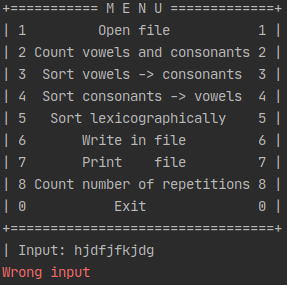
\includegraphics[width=0.5\linewidth]{photo/tests/wrong_input}
	\caption{Ошибочный ввод}
	\label{wrong_input}
\end{figure}

Так как никакой файл не открыт, полный функционал программы недоступен. Попоробуем выбрать пункт меню 2. Ожидается сообщение об ошибке и возврат в меню. Результат на рисунке \ref{no_file_opened}.
\begin{figure}[hpt!]
	\centering
	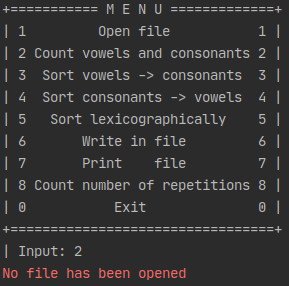
\includegraphics[width=0.5\linewidth]{photo/tests/no_file_opened}
	\caption{Выбор пункта меню, работающего с файлом, при отсутствии открытого файла}
	\label{no_file_opened}
\end{figure}

Откроем загатовленный файл bigfile с помощью пункта меню 1 Open file. Ожидается, что на экран выведутся файлы текущей директории, а после открытия над меню вместо NONE будет отображается имя открытого файла. Результат на рисунке \ref{open}.
\begin{figure}[htp!]
	\centering
	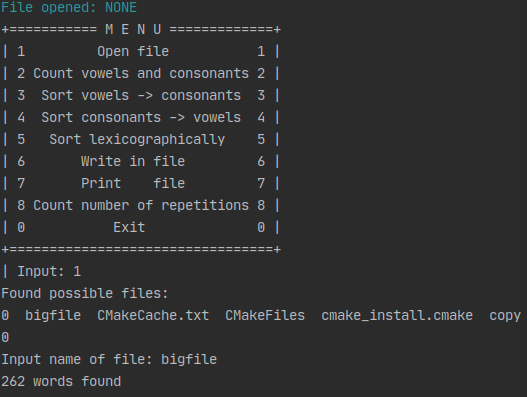
\includegraphics[width=0.7\linewidth]{photo/tests/open}
	\caption{Открытие файла}
	\label{open}
\end{figure}

Выберем 2 пункт меню. Ожидается, что на экран выведется количество гласных и согласных букв в тексте файла, а так же количество символов, которые не являются буквами. Результат на рисунке \ref{countvc}
\begin{figure}[htp!]
	\centering
	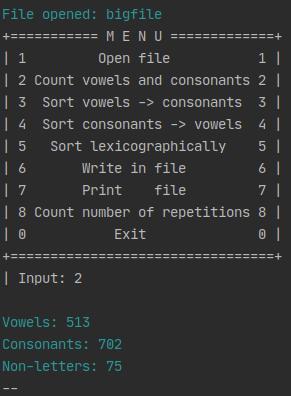
\includegraphics[width=0.5\linewidth]{photo/tests/countvc}
	\caption{Подсчёт количества гласных и согласных букв}
	\label{countvc}
\end{figure}

Выберем 3 пункт меню. Ожидается, что на экран выведется сообщение о том, что изменённое содержимое файла записано в новый файл VtoC.txt. Результат на рисунке \ref{vtoc}. Содержимое файла VtoC.txt на рисунке \ref{vtoc_txt}.
\begin{figure}[htp!]
	\centering
	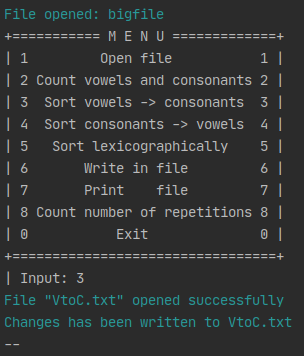
\includegraphics[width=0.5\linewidth]{photo/tests/vtoc}
	\caption{Сортировка от гласных к согласным}
	\label{vtoc}
\end{figure}

\begin{figure}[htp!]
	\centering
	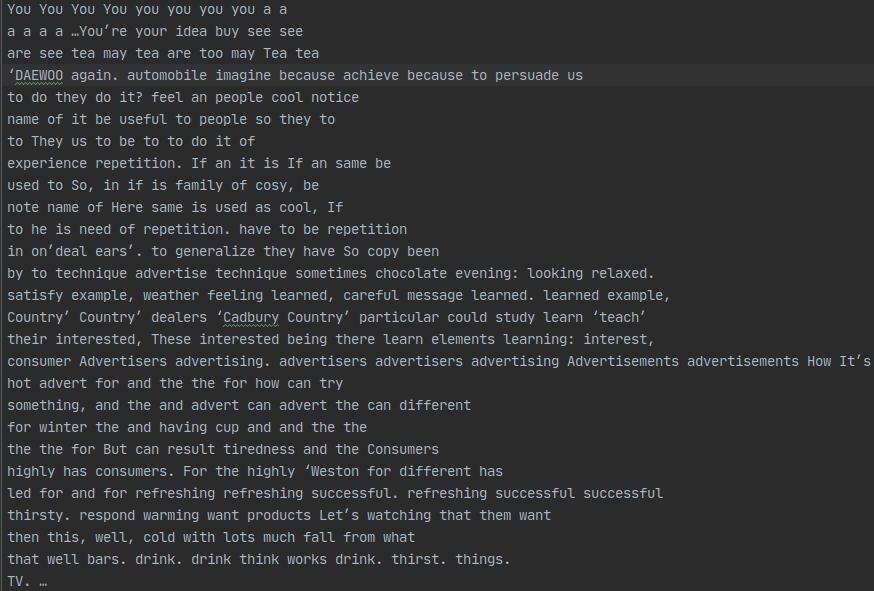
\includegraphics[width=0.9\linewidth]{photo/tests/vtoc_txt}
	\caption{Содержимое файла VtoC.txt}
	\label{vtoc_txt}
\end{figure}

Выберем 4 пункт меню. Ожидается, что на экран выведется сообщение о том, что изменённое содержимое файла записано в новый файл CtoV.txt. Результат на рисунке \ref{ctov}. Содержимое файла CtoV.txt на рисунке \ref{ctov_txt}.
\begin{figure}[htp!]
	\centering
	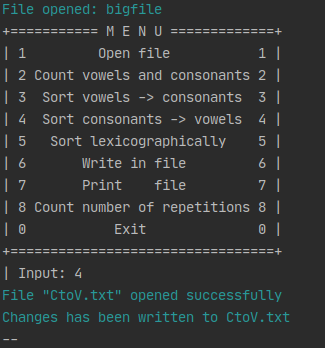
\includegraphics[width=0.5\linewidth]{photo/tests/ctov}
	\caption{Сортировка от согласных к гласным}
	\label{ctov}
\end{figure}

\begin{figure}[htp!]
	\centering
	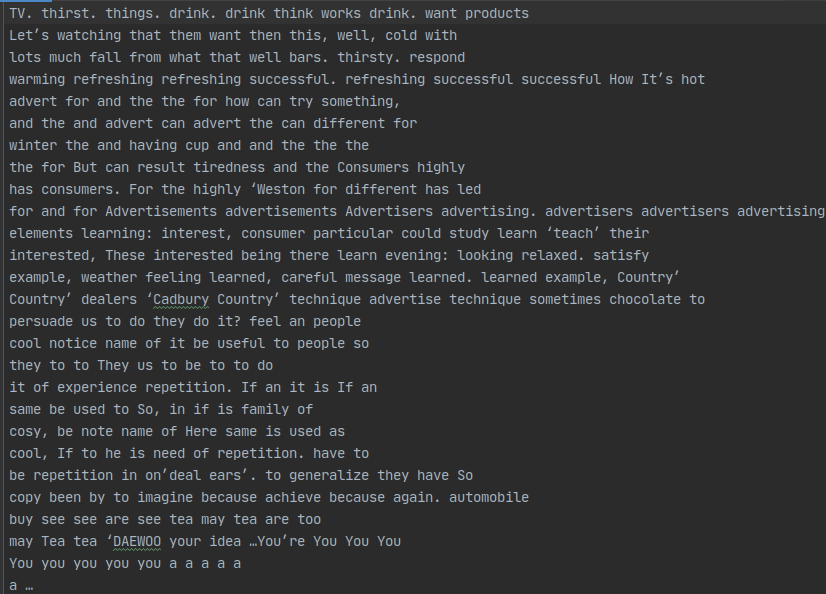
\includegraphics[width=0.9\linewidth]{photo/tests/ctov_txt}
	\caption{Содержимое файла CtoV.txt}
	\label{ctov_txt}
\end{figure}

Выберем 5 пункт меню. Ожидается, что на экран выведется сообщение о том, что изменённое содержимое файла записано в новый файл lex.txt. Результат на рисунке \ref{lex}. Содержимое файла lex.txt на рисунке \ref{lex_txt}.
\begin{figure}[htp!]
	\centering
	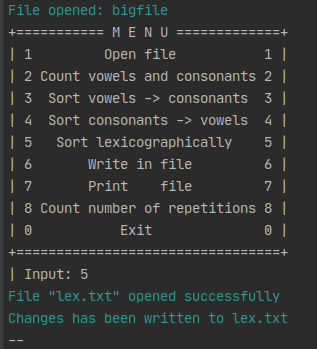
\includegraphics[width=0.5\linewidth]{photo/tests/lex}
	\caption{Сортировка по алфавиту}
	\label{lex}
\end{figure}

\begin{figure}[htp!]
	\centering
	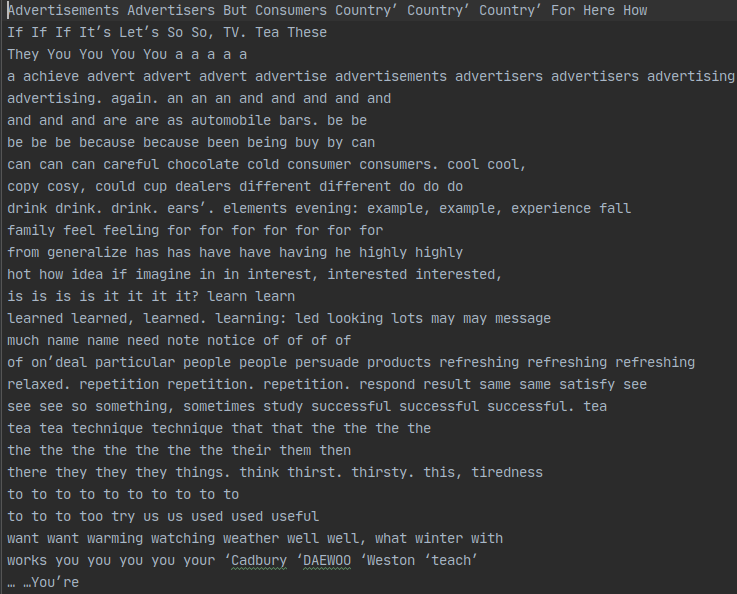
\includegraphics[width=0.9\linewidth]{photo/tests/lex_txt}
	\caption{Содержимое файла lex.txt}
	\label{lex_txt}
\end{figure}

Пункт 6 предлагает пользователю ввести имя файла, в который он хочет записать изменения. 

Выберем 6 пункт меню и попытаемтся открыть существующий файл "0". Ожидается, что на экран выведется сообщение о том, что такой файл уже существует. Отказ от изменений представлен на рисунке \ref{rewrite_no}. Согласие на рисунке \ref{rewrite_yes}. Содержимое файла 0 рисунке \ref{lex_fake_txt}.

\begin{figure}[htp!]
	\centering
	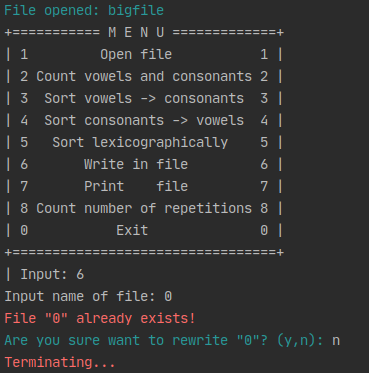
\includegraphics[width=0.5\linewidth]{photo/tests/rewrite_no}
	\caption{Отказ от перезаписи существующего файла}
	\label{rewrite_no}
\end{figure}

\begin{figure}[htp!]
	\centering
	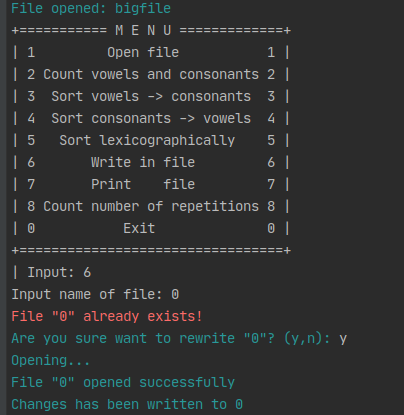
\includegraphics[width=0.5\linewidth]{photo/tests/rewrite_yes}
	\caption{Согласие на перезапись существующего файла}
	\label{rewrite_yes}
\end{figure}

\begin{figure}[htp!]
	\centering
	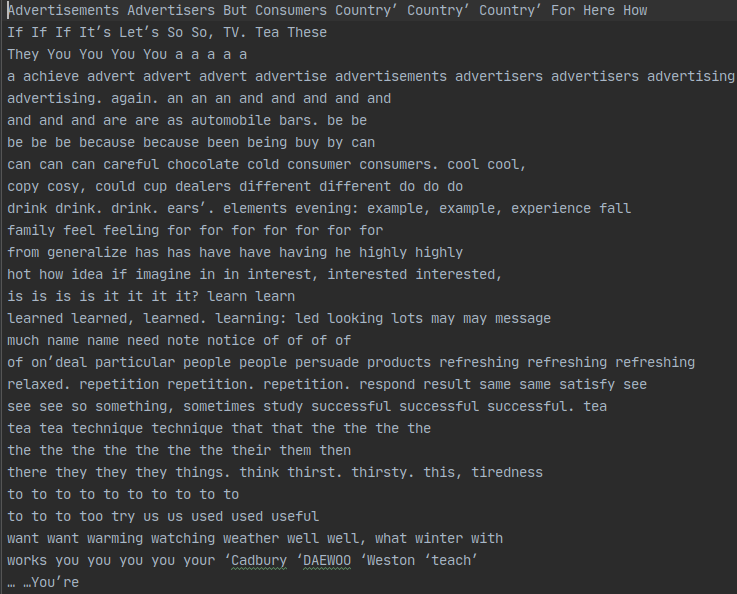
\includegraphics[width=0.9\linewidth]{photo/tests/lex_txt}
	\caption{Содержимое файла 0}
	\label{lex_fake_txt}
\end{figure}

Так как файл слишком большой, он не умещается на экран. Для демонстрации работы пунктов 7-8 откроем другой файл с помощью пункта меню 1 (рисунок \ref{reopen}).

\begin{figure}[htp!]
	\centering
	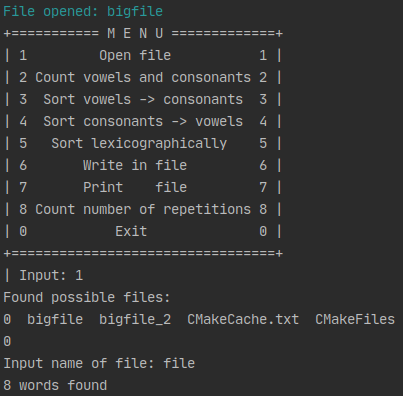
\includegraphics[width=0.5\linewidth]{photo/tests/reopen}
	\caption{Открытие файла при уже открытом другом файле}
	\label{reopen}
\end{figure}

Выберем 7 пункт меню. Ожидается, что на экран выведется содержимое открытого файла. Результат на рисунке \ref{print}

\begin{figure}[htp!]
	\centering
	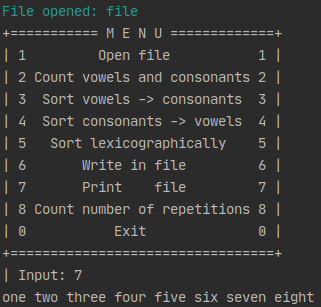
\includegraphics[width=0.5\linewidth]{photo/tests/print}
	\caption{Вывод содержимого файла на экран}
	\label{print}
\end{figure}

Выберем 7 пункт меню. Ожидается, что на экран выведется список уникальных слов, количество их повторений и сообщение о том, что все слова повторяются единожды. Результат на рисунке \ref{count_num_of_reps}. 

\begin{figure}[htp!]
	\centering
	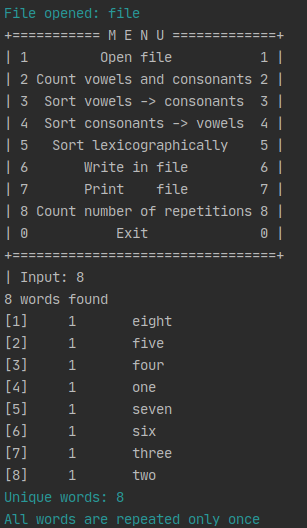
\includegraphics[width=0.5\linewidth]{photo/tests/count_num_of_reps}
	\caption{Вывод количества повторений слов. Все слова повторяются единожды}
	\label{count_num_of_reps}
\end{figure}

Выберем 7 пункт меню при файле, где разные слова имеют разное количество повторений. Ожидается, что на экран выведется список уникальных слов, количество их повторений и сообщение о самом часто встречающемся слове. Результат на рисунках \ref{cnor1} и \ref{cnor2}.

\begin{figure}[htp!]
	\centering
	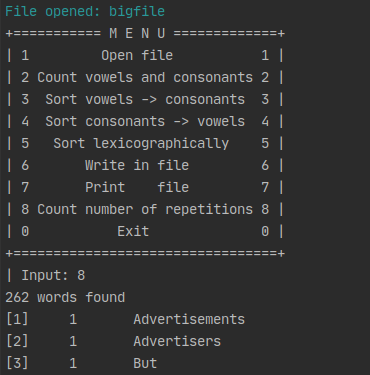
\includegraphics[width=0.5\linewidth]{photo/tests/cnor1}
	\caption{Вывод количества повторений слов (начало)}
	\label{cnor1}
\end{figure}

\begin{figure}[htp!]
	\centering
	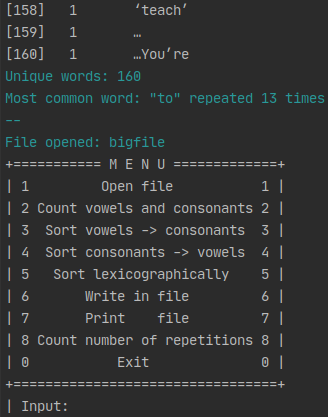
\includegraphics[width=0.5\linewidth]{photo/tests/cnor2}
	\caption{Вывод количества повторений слов (конец)}
	\label{cnor2}
\end{figure}

Выберем 0 пункт меню чтобы завершить программу. Результат на рисунке \ref{exit}.

\begin{figure}[htp!]
	\centering
	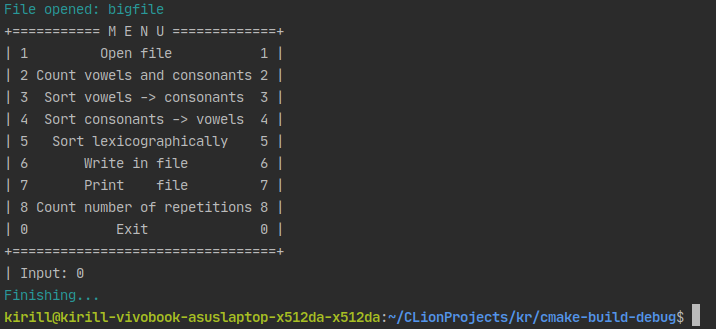
\includegraphics[width=0.5\linewidth]{photo/tests/exit}
	\caption{Выход из программы}
	\label{exit}
\end{figure}

%////////////////////////////////////////////////////////////////////////////////////////////////
%////////////////////////////////////////////////////////////////////////////////////////////////
%////////////////////////////////////////////////////////////////////////////////////////////////
\newpage
\section*{Заключение}
\addcontentsline{toc}{section}{Заключение}
\setcounter{figure}{0}
\begin{comment}
	Своими словами постарайтесь кратко подвести итоги выполненной
	работы: написать, что вы изучили в этой работе и описать полученный
	результат. При написании, опирайтесь на формулировки цели работы и
	существенную часть задания.
\end{comment}

В результате выполнения данной курсовой работы мы закрепили и применили на практике знания, полученные в ходе выполнения лабораторных работ. Реализованная программа соответствует поставленным задачам и безошибочно выполняет свою работу. Функционал программы позволяет не только выполнять вычисления, но и реализует полноценное взаимодействие с пользователем, корректно обрабатывать его запросы и выдавать ему ожидаемый результат. Выполнение данной лабораторной работы позволило углубить наши знания в технологии программирования типовых задач обработки текстовых данных и принципах программной реализации взаимодействия с файлами.


%////////////////////////////////////////////////////////////////////////////////////////////////
%////////////////////////////////////////////////////////////////////////////////////////////////
%////////////////////////////////////////////////////////////////////////////////////////////////
\newpage
\section*{Список использованных сточников}
\setcounter{figure}{0}
\addcontentsline{toc}{section}{Список использованных сточников}
\begin{comment}
	1 Страуструп Б. Язык программирования C++. Специальное издание. - М.:
	Бином; СПб.: Невский диалект, 2008 - 1104 с.
	2 Дейтел Х.М., Дейтел П.Дж. Как программировать на C++. 5-е издание.
	Перевод с англ. - М.: ООО «Бином-Пресс», 2008 - 1456 с.
	3 Хигай А.Г., Зуев И.С., Грушвицкий Р.И. Программирование на языке С в
	среде Borland 3.1: Методические указания к лабораторным работам по
	дисциплинам
	«Информатика»,
	«Программирование».
	-
	СПб.:
	Издательство СПбГЭТУ «ЛЭТИ», 2006
	4 Калмычков
	В.А.,
	Чугунов
	Л.А.
	Представление
	и
	обработка
	математических данных на языке С++: Учебное пособие. - СПб.:
	Издательтство СПбГЭТУ «ЛЭТИ», 2010
	5 Ивановский С.А., Калмычкова В.А., Лисс А.А. Разработка корректных
	программ: Практикум по программированию. - СПб.: Издательство
	СПбГЭТУ «ЛЭТИ», 2001
	6 Литвинова Л.А. Методические указания к лабораторным занятиям по
	дисциплине «Алгоритмизация и программирование» (раздел «Решение
	задач в среде Turbo-Pascal») для студентов направления 6050202
	«Автоматизация и компьютерно-интегрированные технологии» дневной
	формы обучения. - Севастополь: Издательство СевНТУ, 2011 - 36 с.
	7 Павловская Т.А. С/С++. Программирование на языке высокого уровня.
	СПб.: Лидер, 2010 - 461 с.
	8 Павловская Т.А., Щипак Ю.А. С/С++. Структурное программирование:
	Практикум. - СПб.: Питер, 2004, 2005, 2007 - 240 с.
\end{comment}

\begin{list}{[1]}{}
	\item Заголовочный файл стандартной библиотеки <string> — cppreference.com. (n.d.). Retrieved May 15, 2020, from https://ru.cppreference.com/w/cpp/header/string
\end{list}

\begin{list}{[2]}{}
	\item std::basic\_fstream — cppreference.com. (n.d.). Retrieved May 15, 2020, from https://ru.cppreference.com/w/cpp/io/basic\_fstream
\end{list}

\begin{list}{[3]}{}
	\item Лексикографический порядок — Википедия. (n.d.). Retrieved May 15, 2020, from https://ru.wikipedia.org/wiki/Лексикографический\_порядок
\end{list}

\begin{list}{[4]}{}
	\item std::sort — cppreference.com. (n.d.). Retrieved May 15, 2020, from https://ru.cppreference.com/w/cpp/algorithm/sort
\end{list}

\begin{comment}
https://ru.cppreference.com/w/cpp/header/string

https://ru.cppreference.com/w/cpp/algorithm/sort

https://ru.cppreference.com/w/cpp/io/basic\_fstream

https://ru.wikipedia.org/wiki/\%D0\%9B\%D0\%B5\%D0\%BA\%D1\%81\%D0\%B8\%D0\%BA\%D0\%BE\%D0\%B3\%D1\%80\%D0\%B0\%D1\%84\%D0\%B8\%D1\%87\%D0\%B5\%D1\%81\%D0\%BA\%D0\%B8\%D0\%B9\_\%D0\%BF\%D0\%BE\%D1\%80\%D1\%8F\%D0\%B4\%D0\%BE\%D0\%BA

https://ru.wikipedia.org/wiki/%D0%9B%D0%B5%D0%BA%D1%81%D0%B8%D0%BA%D0%BE%D0%B3%D1%80%D0%B0%D1%84%D0%B8%D1%87%D0%B5%D1%81%D0%BA%D0%B8%D0%B9_%D0%BF%D0%BE%D1%80%D1%8F%D0%B4%D0%BE%D0%BA
\end{comment}

%////////////////////////////////////////////////////////////////////////////////////////////////
%////////////////////////////////////////////////////////////////////////////////////////////////
%////////////////////////////////////////////////////////////////////////////////////////////////
\newpage
\section*{Приложение А\\ Листинг программного кода}
\setcounter{figure}{0}
\addcontentsline{toc}{section}{Приложение А  Исходный код программы}
\subsection*{main.cpp}
\addcontentsline{toc}{subsection}{main.cpp}
\lstinputlisting{src/main.cpp}
\newpage
\subsection*{openFile.cpp}
\addcontentsline{toc}{subsection}{openFile.cpp}
\lstinputlisting{src/openFile.cpp}
\newpage
\subsection*{openFile.h}
\addcontentsline{toc}{subsection}{openFile.h}
\lstinputlisting{src/openFile.h}
\newpage
\subsection*{countVC.cpp}
\addcontentsline{toc}{subsection}{countVC.cpp}
\lstinputlisting{src/countVC.cpp}
\newpage
\subsection*{countVC.h}
\addcontentsline{toc}{subsection}{countVC.h}
\lstinputlisting{src/countVC.h}
\newpage
\subsection*{writeFile.cpp}
\addcontentsline{toc}{subsection}{writeFile.cpp}
\lstinputlisting{src/writeFile.cpp}
\newpage
\subsection*{writeFile.h}
\addcontentsline{toc}{subsection}{writeFile.h}
\lstinputlisting{src/writeFile.h}
\newpage
\subsection*{countWords.cpp}
\addcontentsline{toc}{subsection}{countWords.cpp}
\lstinputlisting{src/countWords.cpp}
\newpage
\subsection*{countWords.h}
\addcontentsline{toc}{subsection}{countWords.h}
\lstinputlisting{src/countWords.h}
\newpage
\subsection*{sortVC.cpp}
\addcontentsline{toc}{subsection}{sortVC.cpp}
\lstinputlisting{src/sortVC.cpp}
\newpage
\subsection*{sortVC.h}
\addcontentsline{toc}{subsection}{sortVC.h}
\lstinputlisting{src/sortVC.h}
\newpage
\subsection*{printFile.cpp}
\addcontentsline{toc}{subsection}{printFile.cpp}
\lstinputlisting{src/printFile.cpp}
\newpage
\subsection*{printFile.h}
\addcontentsline{toc}{subsection}{printFile.h}
\lstinputlisting{src/printFile.h}
\newpage
\subsection*{Colors.h}
\addcontentsline{toc}{subsection}{Colors.h}
\lstinputlisting{src/Colors.h}
\newpage
\subsection*{calck.cpp}
\addcontentsline{toc}{subsection}{calck.cpp}
\lstinputlisting{src/calck.cpp}
\newpage
\subsection*{calck.h}
\addcontentsline{toc}{subsection}{calck.h}
\lstinputlisting{src/calck.h}
\newpage
\end{document}